\documentclass[10pt,a4paper]{article}

% Encodage et langue
\usepackage[T1]{fontenc}
\usepackage[utf8]{inputenc}
\usepackage[french]{babel}

% Maths
\usepackage{amsmath,amssymb,amsthm}

% Figures et tableaux
\usepackage{graphicx}
\usepackage{booktabs}
\usepackage{caption}
\usepackage{subcaption}

% Mise en page
\usepackage[a4paper,margin=2.5cm]{geometry}
\usepackage{setspace}
\onehalfspacing

% Liens
\usepackage[colorlinks=true,
            linkcolor=blue,
            citecolor=blue,
            urlcolor=blue]{hyperref}


% Blocs de code
\usepackage{xcolor}
\usepackage{listings}

\definecolor{codegreen}{rgb}{0,0.6,0}
\definecolor{codegray}{rgb}{0.5,0.5,0.5}
\definecolor{codepurple}{rgb}{0.58,0,0.82}

\lstdefinestyle{mystyle}{
    language=Python,
    basicstyle=\ttfamily\small,
    keywordstyle=\color{blue}\bfseries,
    commentstyle=\color{codegreen}\itshape,
    stringstyle=\color{codepurple},
    numbers=left,
    numberstyle=\tiny\color{codegray},
    frame=single,
    breaklines=true,
    showstringspaces=false
}

\lstset{style=mystyle}

% Informations du document
\title{\textbf{Meilleurs paramètres pour A--HNC}}
\author{Amyne KADDOURI}
\date{\today}

% Pas d'indentation
\setlength{\parindent}{0pt}

\begin{document}

\maketitle

\tableofcontents
\newpage

%--------------------------------------------------

\section{A savoir}

Dans mon implémentation de la fonction $V$ en python, j'ai imposé 
$V_{sh}(R,\theta)=G(R,\theta)e^{D(\theta)-B(\theta)R}$.\\

Les fits, calculs d'erreurs et figures ont été fait à partir de toutes les 
données de référence fournies dans le fichier "\verb|redgrid.dat|" pour le cas
Ar-HNC.\\

J'ai sélectionné les paramètres qui présentaient les meilleurs erreurs et qui
reproduisaient le mieux les données ab initio (graphiquement principalement)
obtenus à l'aide des méthodes (\verb|curve_fit| et \verb|least_squares|).
Je me suis assuré que les valeurs de c0, c1, c2 et c3 respectaient bien la
même échelle et (au moins) le même signe que les paramètres donnés par 
Toczylowski pour Ar-HCN.\\

\section{Les 3 jeux de paramètres}

\subsection{Valeurs obtenues}

\begin{table}[ht]
\centering
\caption{Paramètres 1}
\label{params_cf_trf_sigma}
\resizebox{\textwidth}{!}{%
\begin{tabular}{lrrrrrr}
\toprule
 & 0 & 1 & 2 & 3 & 4 & 5 \\
\midrule
$b$    & 1.3927514645113     & 0.0969300220323 &-0.0598408365993     & 0.0979666320780 & 0.0440331249725 &-0.0066773573730 \\
$c$    &-135783.58642776     &-325692.43447538 &-57995.311054132     &-125784.84697654 &  &  \\
$d$    & 14.356222526628     & 1.2155113608982 & 1.1171693978112     & 0.4725050499800 & 0.2654722356128 & 0.0397397126798 \\
$g_0$  & 0.0421957569618     &-0.0743663336295 & 0.0044449246699     &-0.0055690533186 & 0.0510967140603 &-0.0110267889605 \\
$g_1$  & 0.0012035409107     & 0.0230019854597 & 0.0016336165358     &-0.0014389874416 &-0.0208051820470 & 0.0056295386237 \\
$g_2$  &-0.0014415287347     &-0.0031206461923 &-0.0005977968133     & 0.0011482862886 & 0.0027666079533 &-0.0009802729077 \\
$g_3$  & 0.0000769984960     & 0.0001784250246 & 0.0000445011209     &-0.0001171508711 &-0.0001207857249 & 0.0000577998328 \\
\bottomrule
\end{tabular}%
}
\end{table}

\begin{table}[ht]
\centering
\caption{Paramètres 2}
\label{params_ls_sigma_final}
\resizebox{\textwidth}{!}{%
\begin{tabular}{lrrrrrr}
\toprule
 & 0 & 1 & 2 & 3 & 4 & 5 \\
\midrule
$b$    & 1.9387866839570 &-0.0223991224994 &-0.0509154407913 & 0.182868733272 & 0.1501564500171 &-0.0137991355166 \\
$c$    &-167830.37667653 &-53.992794635238 &-113083.72444830 &-71.61804480350 &  &  \\
$d$    & 15.815015606625 & 2.0803397264399 & 1.2276661118939 & 1.476489725164 & 1.0239260345891 &-0.0687383269251 \\
$g_0$  &-0.2172379299951 & 0.6018686726955 &-0.9176628958772 & 0.948494926539 &-0.5172129279637 & 0.1542049190582 \\
$g_1$  & 0.0714244569620 &-0.2190836144982 & 0.4082100434331 &-0.482755537952 & 0.2665181426544 &-0.0730598863798 \\
$g_2$  & 0.0058467888002 & 0.0037123730282 &-0.0454412925179 & 0.072062821573 &-0.0414597559586 & 0.0108484897026 \\
$g_3$  &-0.0009159804243 & 0.0007835671754 & 0.0019035531089 &-0.003774079765 & 0.0022020804985 &-0.0005461266426 \\
\bottomrule
\end{tabular}%
}
\end{table}

\begin{table}[ht]
\centering
\caption{Paramètres 3}
\label{params_ls_bounded}
\resizebox{\textwidth}{!}{%
\begin{tabular}{lcccccc}
\toprule
 & 0 & 1 & 2 & 3 & 4 & 5 \\
\midrule
$b$   & 1.8874319477762 &-0.0088557975081 &-0.0076878652357 & 0.1634650917639 & 0.1461768669673 & 0.0001286231021 \\
$c$   &-164473.38854722 &-4238.2611988215 &-110793.91739105 &-4249.3463047611 &  &  \\
$d$   & 15.591793713767 & 2.1309189103932 & 1.4595744806007 & 1.3633708258703 & 1.0049872024066 & 0.0110106374830 \\
$g_0$ &-0.2363619657742 & 0.6113451840448 &-0.8591649325880 & 0.8403833810070 &-0.4338937932884 & 0.1295084478368 \\
$g_1$ & 0.0887705592254 &-0.2335273580799 & 0.3782962964383 &-0.4227921331950 & 0.2200463550578 &-0.0591965211768 \\
$g_2$ & 0.0022793743057 & 0.0070174284118 &-0.0409139856048 & 0.0623736729987 &-0.0337105162744 & 0.0084571606460 \\
$g_3$ &-0.0008210883057 & 0.0007805311972 & 0.0015836338437 &-0.0032652944208 & 0.0017922273601 &-0.0004134049294 \\
\bottomrule
\end{tabular}%
}
\end{table}

\newpage{}
\subsection{Détails des méthodes}

\subsubsection{Premier jeu (Table~\ref{params_cf_trf_sigma})}

\begin{itemize}
  \item Fonction : \verb|curve_fit|
  \item Paramètres initiaux p0 : paramètres optimaux de Ar-HCN pour les données
    ab-initio de Toczylowski (pour avoir un point de départ)
  \item \verb|method='trf'|
  \item \verb|sigma=V_mEh| où \verb|V_mEh| est le vecteur contenant les données
    de référence
\end{itemize}

\subsubsection{Deuxième jeu (Table~\ref{params_ls_sigma_final})}

\begin{itemize}
  \item Fonction : \verb|least_squares|
  \item Paramètres initiaux : Table~\ref{params_cf_trf_sigma}
  \item \verb|method='trf'|
  \item \verb|loss='soft_l1'|
  \item \verb|f_scale=0.1|
  \item Fonction résidus : \verb|residuals_final|
\end{itemize}

\begin{lstlisting}[language=Python, caption={Fonction résidus}, label={lst:residuals_final}]
E_range = np.max(V_mEh) - np.min(V_mEh)
sigma_final = np.maximum(np.abs(V_mEh), 0.02 * E_range)

def residuals_final(p, R, Theta, E_ref, sigma):
    return (V_opt_de(p, R, Theta) - E_ref) / sigma
\end{lstlisting}

Avec \verb|V_opt_de| qui est une version de l'implémentation de V dans laquelle
une conversion est appliquée sur les paramètres c pour stabiliser numériquement
la méthode d'optimisation : $c_{de}=\log_{10}(c_{reel})$.

\subsubsection{Troisième jeu (Table~\ref{params_ls_bounded})}

\begin{itemize}
  \item Fonction : \verb|least_squares|
  \item Paramètres initiaux : Table~\ref{params_cf_trf_sigma}
  \item \verb|method='trf'|
  \item \verb|loss='soft_l1'|
  \item \verb|f_scale=0.1|
  \item Fonction résidus : \verb|residuals_final|
  \item \verb|bounds=(inf,sup)| : on applique un intervale pour éviter d'avoir :
    c$_{0}$, c$_{2}$ de l'ordre de $-10^6$ et c$_{1}$, c$_{3}$ de l'ordre de $-10^1$
\end{itemize}

\newpage{}
\section{Erreurs obtenues en comparaison aux données de référence}

\begin{table}[ht]
\centering
\caption{Erreurs globales}
\label{erreurs_global}
\resizebox{\textwidth}{!}{%

\begin{tabular}{lrrrrrrrr}
\toprule
 & R² & RMSE (cm-1) & MAE (cm-1) & Relative Max (\%) & Relative Moyenne (\%) & Absolue Max (cm-1) & Absolue Moyenne (cm-1) & Score Régularité \\
\midrule
Paramètres \ref{params_cf_trf_sigma} & 0.975292 & 1793.545540 & 136.890764 & 38.508793 & 0.243320 & 98073.349786 & 136.890764 & 83 \\
Paramètres \ref{params_ls_sigma_final} & 0.999838 & 145.416083 & 12.418732 & 6.040209 & 0.037614 & 6843.420117 & 12.418732 & 81 \\
Paramètres \ref{params_ls_bounded} & 0.999820 & 153.207453 & 12.285500 & 6.815061 & 0.034710 & 7665.298152 & 12.285500 & 74 \\
\bottomrule
\end{tabular}%
}
\end{table}

Vous trouverez en annexe le tableau pour tous les paramètres que j'ai calculé (Table~\ref{erreurs_all}). \\


\begin{itemize}
  \item \textbf{R$^2$} : sans unité, indique sur la tendance globale
  \item \textbf{RMSE} : Racine de l’erreur quadratique moyenne (ici en cm$^{-1}$), mise
    en valeur des erreurs importantes
  \item \textbf{MAE} : Erreur absolue moyenne (ici en cm$^{-1}$), mise en
    valeur de l'erreur moyenne
  \item \textbf{Relative Max} : $100\times\max(\frac{|V_{fit}-V_{ref}|}{|V_{ref}|+ 0.02\times(\max(V_{ref})-\min(V_{ref}))})$
  \item \textbf{Relative Moyenne} : $100\times\text{mean}(\frac{|V_{fit}-V_{ref}|}{|V_{ref}|+ 0.02\times(\max(V_{ref})-\min(V_{ref}))})$
  \item \textbf{Absolue Max} : $\max(|V_{fit}-V_{ref}|)$
  \item \textbf{Absolue Moyenne} : $\text{mean}(|V_{fit}-V_{ref}|)$
  \item \textbf{Score Régularité} : Pénalisation des oscilations ne correspondant pas aux données de référence. 
    On vise un score bas.
\end{itemize}

\begin{table}[ht]
\centering
\caption{Erreurs par intervalle de $\theta$ pour Paramètres \ref{params_cf_trf_sigma}}
\label{tab:erreurs_theta_1}
\resizebox{\textwidth}{!}{%
\begin{tabular}{lrrr}
\toprule
$\theta$ (degrés) & RMSE (cm$^{-1}$) & Erreur relative max. (\%) & Erreur absolue max. (cm$^{-1}$) \\
\midrule
$[0,10]$     & 6273.749 & 27.80 & 98073.350 \\
$[10,20]$    & 1676.777 & 14.75 & 37799.983 \\
$[20,30]$    & 379.498  & 3.67  & 3488.934 \\
$[30,40]$    & 321.704  & 6.89  & 4513.214 \\
$[40,50]$    & 526.820  & 10.75 & 5720.395 \\
$[50,60]$    & 348.539  & 9.79  & 4494.486 \\
$[60,70]$    & 151.062  & 6.57  & 2303.750 \\
$[70,80]$    & 20.827   & 0.82  & 216.924 \\
$[80,90]$    & 22.600   & 1.01  & 264.041 \\
$[90,100]$   & 23.903   & 1.46  & 378.743 \\
$[100,110]$  & 41.755   & 1.94  & 543.911 \\
$[110,120]$  & 81.157   & 4.37  & 1434.929 \\
$[120,130]$  & 254.541  & 10.73 & 4394.437 \\
$[130,140]$  & 486.728  & 15.60 & 7665.610 \\
$[140,150]$  & 1035.158 & 26.64 & 16954.269 \\
$[150,160]$  & 1652.269 & 30.26 & 25310.709 \\
$[160,170]$  & 2227.226 & 33.73 & 31795.118 \\
$[170,180]$  & 1715.479 & 24.85 & 27444.206 \\
\bottomrule
\end{tabular}%
}
\end{table}

\begin{table}[ht]
\centering
\caption{Erreurs par intervalle de $\theta$ pour Paramètres \ref{params_ls_sigma_final}}

\label{tab:erreurs_theta_2}
\resizebox{\textwidth}{!}{%
\begin{tabular}{lrrr}
\toprule
$\theta$ (degrés) & RMSE (cm$^{-1}$) & Erreur relative max. (\%) & Erreur absolue max. (cm$^{-1}$) \\
\midrule
$[0,10]$     & 201.855 & 1.19 & 4190.949 \\
$[10,20]$    & 206.288 & 1.76 & 3690.446 \\
$[20,30]$    & 104.797 & 1.78 & 2112.848 \\
$[30,40]$    & 35.043  & 0.99 & 734.362 \\
$[40,50]$    & 16.609  & 0.47 & 242.343 \\
$[50,60]$    & 16.117  & 0.94 & 385.374 \\
$[60,70]$    & 25.608  & 1.55 & 507.766 \\
$[70,80]$    & 10.199  & 0.78 & 215.827 \\
$[80,90]$    & 6.497   & 0.30 & 54.351 \\
$[90,100]$   & 7.010   & 0.39 & 76.971 \\
$[100,110]$  & 5.754   & 0.26 & 70.875 \\
$[110,120]$  & 9.831   & 0.43 & 125.363 \\
$[120,130]$  & 23.972  & 0.75 & 263.443 \\
$[130,140]$  & 55.277  & 1.26 & 566.596 \\
$[140,150]$  & 61.442  & 1.73 & 1102.629 \\
$[150,160]$  & 81.545  & 2.34 & 1960.831 \\
$[160,170]$  & 291.110 & 5.51 & 5190.925 \\
$[170,180]$  & 405.970 & 5.70 & 6843.475 \\
\bottomrule
\end{tabular}%
}
\end{table}

\begin{table}[ht]
\centering
\caption{Erreurs par intervalle de $\theta$ pour Paramètres \ref{params_ls_bounded}}
\label{tab:erreurs_theta_3}
\resizebox{\textwidth}{!}{%
\begin{tabular}{lrrr}
\toprule
Intervalle $\theta$ & RMSE (cm$^{-1}$) & Erreur relative max. (\%) & Erreur absolue max. (cm$^{-1}$) \\
\midrule
$[0,10]$     & 171.457 & 1.02 & 3591.053 \\
$[10,20]$    & 196.275 & 1.66 & 3514.439 \\
$[20,30]$    & 104.885 & 1.78 & 2118.221 \\
$[30,40]$    & 31.009  & 0.91 & 675.994 \\
$[40,50]$    & 18.824  & 0.61 & 315.153 \\
$[50,60]$    & 14.668  & 0.90 & 368.315 \\
$[60,70]$    & 23.910  & 1.47 & 482.181 \\
$[70,80]$    & 9.391   & 0.76 & 210.996 \\
$[80,90]$    & 5.121   & 0.23 & 52.057 \\
$[90,100]$   & 5.928   & 0.33 & 64.445 \\
$[100,110]$  & 5.365   & 0.28 & 75.742 \\
$[110,120]$  & 9.992   & 0.48 & 145.333 \\
$[120,130]$  & 20.458  & 0.71 & 260.338 \\
$[130,140]$  & 47.663  & 1.05 & 473.020 \\
$[140,150]$  & 68.826  & 2.24 & 1425.982 \\
$[150,160]$  & 90.313  & 2.50 & 2093.162 \\
$[160,170]$  & 266.177 & 5.24 & 4941.301 \\
$[170,180]$  & 481.583 & 6.38 & 7665.332 \\
\bottomrule
\end{tabular}%
}
\end{table}

\clearpage{}
\begin{figure}[H]
    \centering
    \caption{Erreurs pour chaque point en échelle logarithmique pour Paramètres \ref{params_cf_trf_sigma}}
    \begin{subfigure}{0.45\textwidth}
        \centering
        \caption{Erreur absolue (cm$^{-1}$)}
        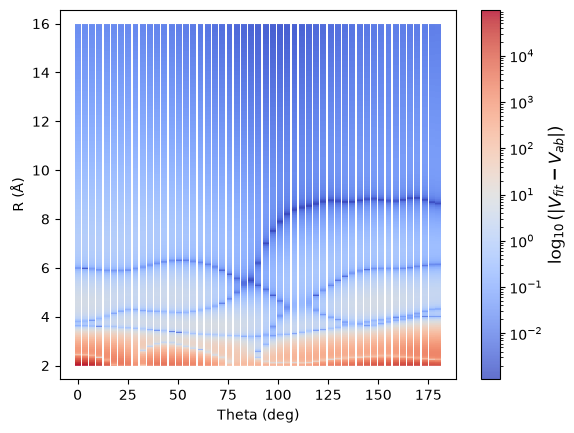
\includegraphics[width=\linewidth]{../Figures/HNC/log_err_abs1.png}
    \end{subfigure}
    \begin{subfigure}{0.45\textwidth}
        \centering
        \caption{Erreur relative (\%)}
        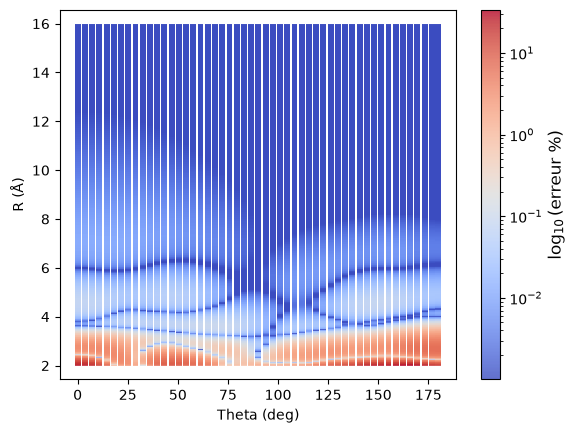
\includegraphics[width=\linewidth]{../Figures/HNC/log_err_rel1.png}
    \end{subfigure}
\end{figure}

\begin{figure}[H]
    \centering
    \caption{Erreurs pour chaque point en échelle logarithmique pour Paramètres \ref{params_ls_sigma_final}}
    \begin{subfigure}{0.45\textwidth}
        \centering
        \caption{Erreur absolue (cm$^{-1}$)}
        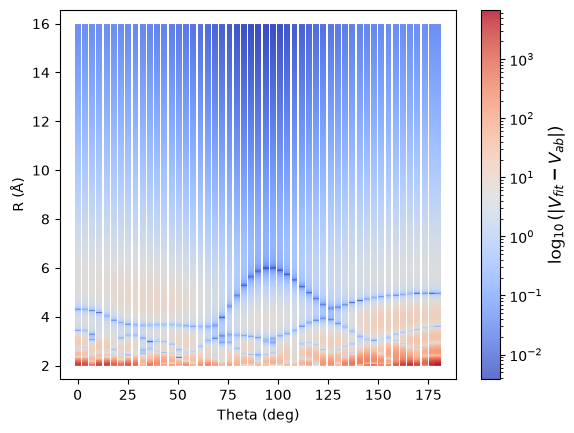
\includegraphics[width=\linewidth]{../Figures/HNC/log_err_abs2.png}
    \end{subfigure}
    \begin{subfigure}{0.45\textwidth}
        \centering
        \caption{Erreur relative (\%)}
        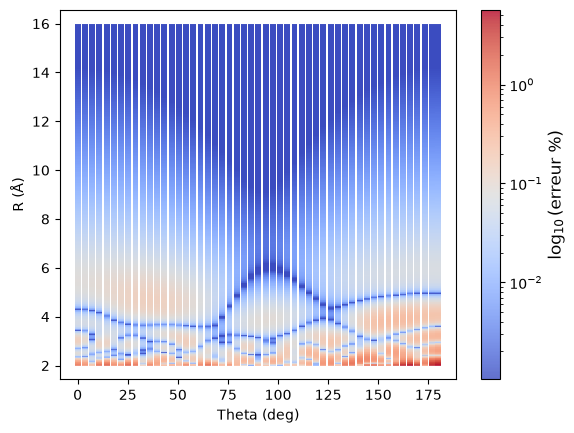
\includegraphics[width=\linewidth]{../Figures/HNC/log_err_rel2.png}
    \end{subfigure}
\end{figure}

\begin{figure}[H]
    \centering
    \caption{Erreurs pour chaque point en échelle logarithmique pour Paramètres \ref{params_ls_bounded}}
    \begin{subfigure}{0.45\textwidth}
        \centering
        \caption{Erreur absolue (cm$^{-1}$)}
        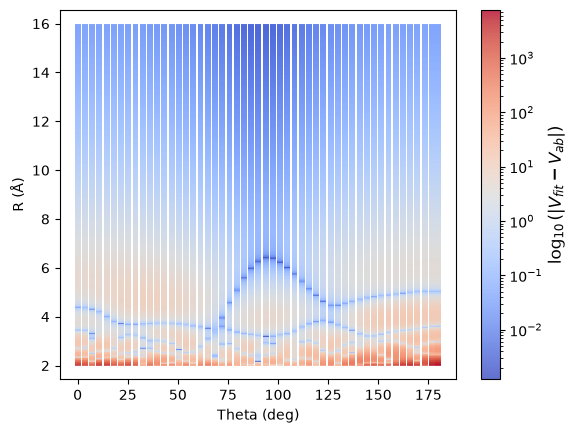
\includegraphics[width=\linewidth]{../Figures/HNC/log_err_abs3.png}
    \end{subfigure}
    \begin{subfigure}{0.45\textwidth}
        \centering
        \caption{Erreur relative (\%)}
        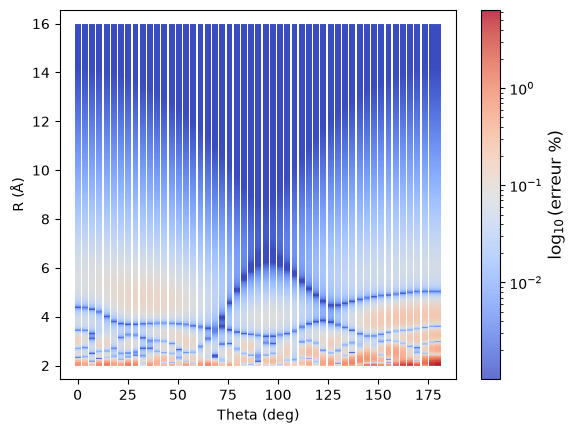
\includegraphics[width=\linewidth]{../Figures/HNC/log_err_rel3.png}
    \end{subfigure}
\end{figure}

\clearpage{}
\newpage{}
\section{Contour plot}

\begin{figure}[h]
    \centering
    \caption{Contour plot de de la surface d'énergies potentielles en cm$^{-1}$ pour Ar--HNC linéaire quand $\theta=0$°}
    \begin{subfigure}{0.49\textwidth}
        \centering
        \caption{Données de référence}
        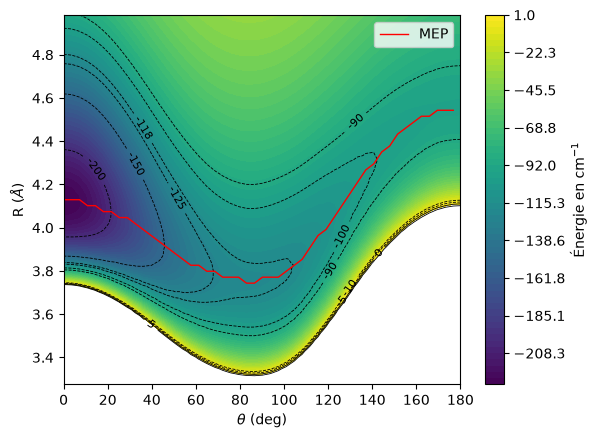
\includegraphics[width=\linewidth]{../Figures/HNC/contour-ref.png}
    \end{subfigure}
    \begin{subfigure}{0.49\textwidth}
        \centering
        \caption{Paramètres \ref{params_cf_trf_sigma}}
        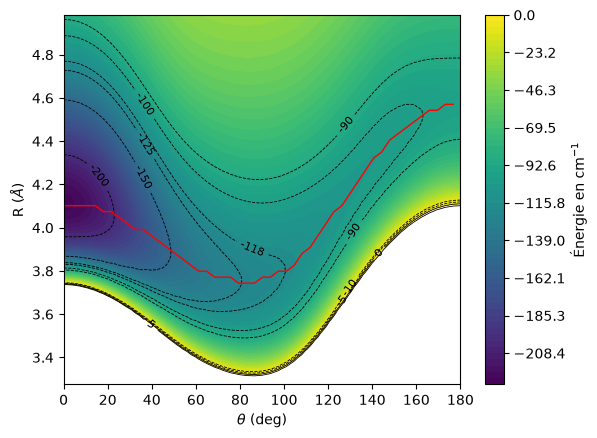
\includegraphics[width=\linewidth]{../Figures/HNC/contour1.png}
    \end{subfigure}
    \begin{subfigure}{0.49\textwidth}
        \centering
        \caption{Paramètres \ref{params_ls_sigma_final}}
        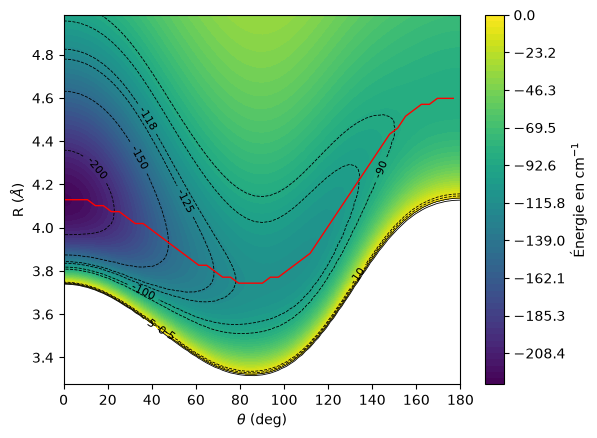
\includegraphics[width=\linewidth]{../Figures/HNC/contour2.png}
    \end{subfigure}
    \begin{subfigure}{0.49\textwidth}
        \centering
        \caption{Paramètres \ref{params_ls_bounded}}
        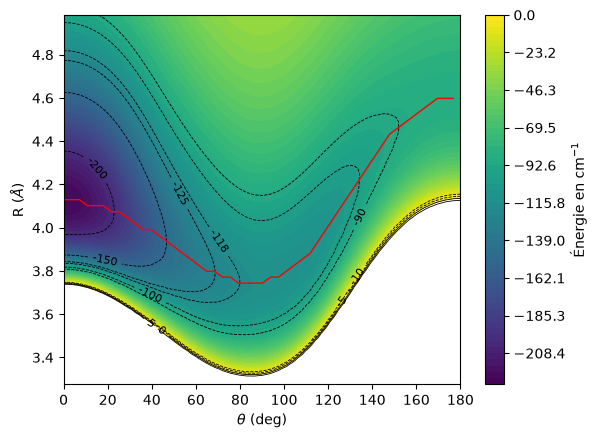
\includegraphics[width=\linewidth]{../Figures/HNC/contour3.png}
    \end{subfigure}
\end{figure}

\newpage{}
\section{Minimums Energy Paths}

\begin{figure}[h]
    \centering
    \caption{Minimums Energy Paths en cm$^{-1}$ pour Ar--HNC linéaire quand $\theta=0$°}
    \begin{subfigure}{0.49\textwidth}
        \centering
        \caption{Données de référence}
        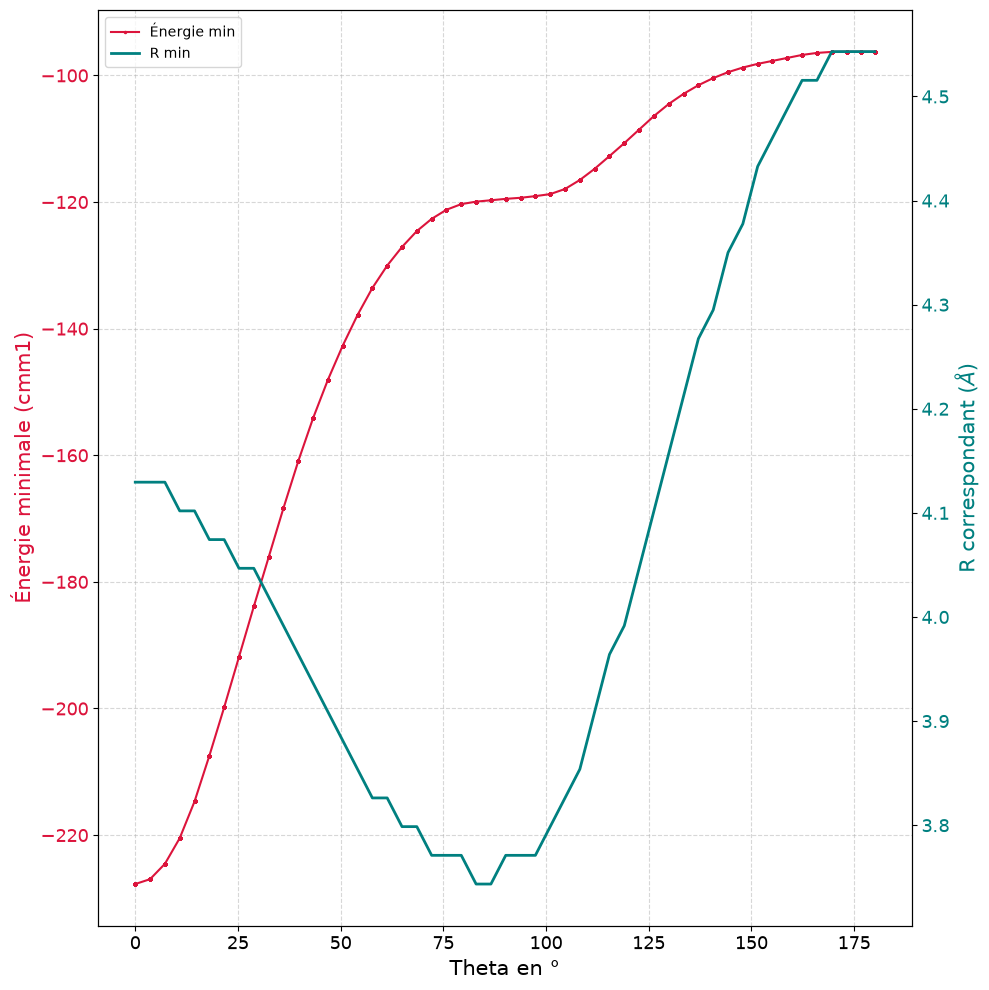
\includegraphics[width=\linewidth]{../Figures/HNC/MEP-ref.png}
    \end{subfigure}
    \begin{subfigure}{0.49\textwidth}
        \centering
        \caption{Paramètres \ref{params_cf_trf_sigma}}
        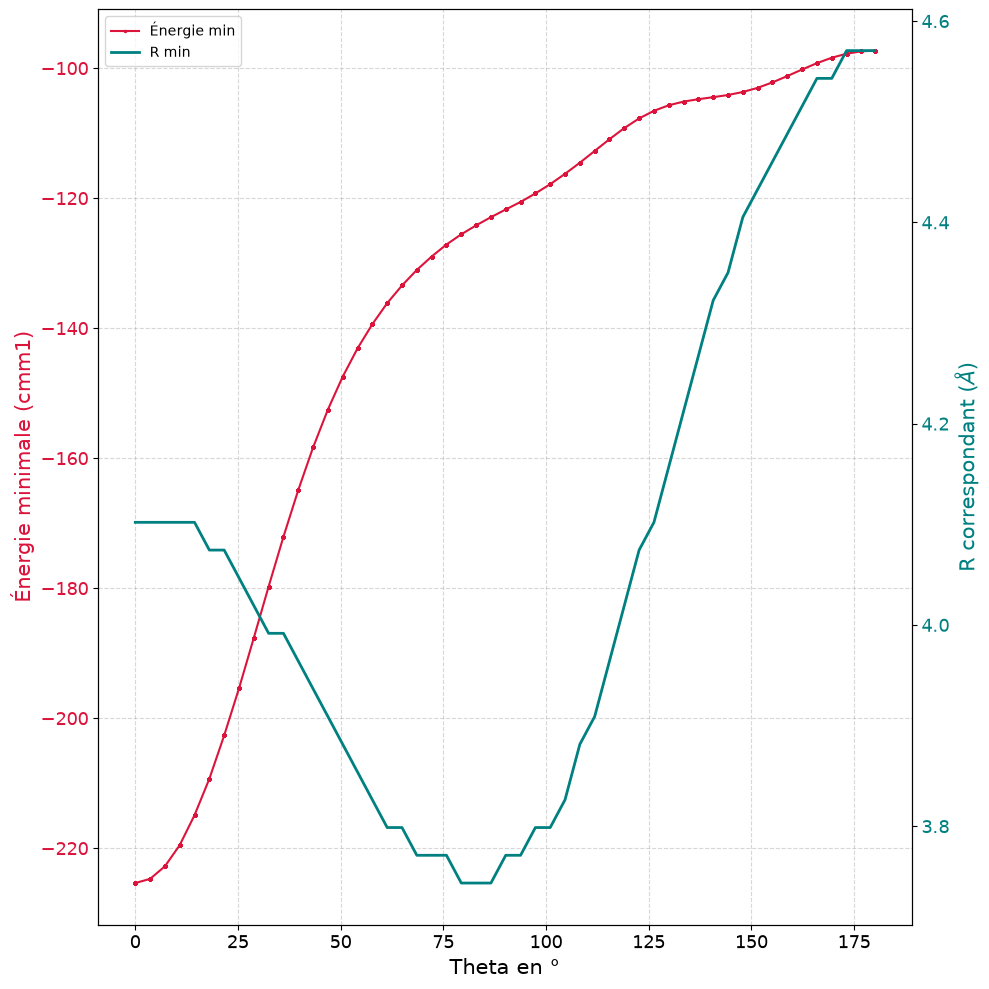
\includegraphics[width=\linewidth]{../Figures/HNC/MEP1.png}
    \end{subfigure}
    \begin{subfigure}{0.49\textwidth}
        \centering
        \caption{Paramètres \ref{params_ls_sigma_final}}
        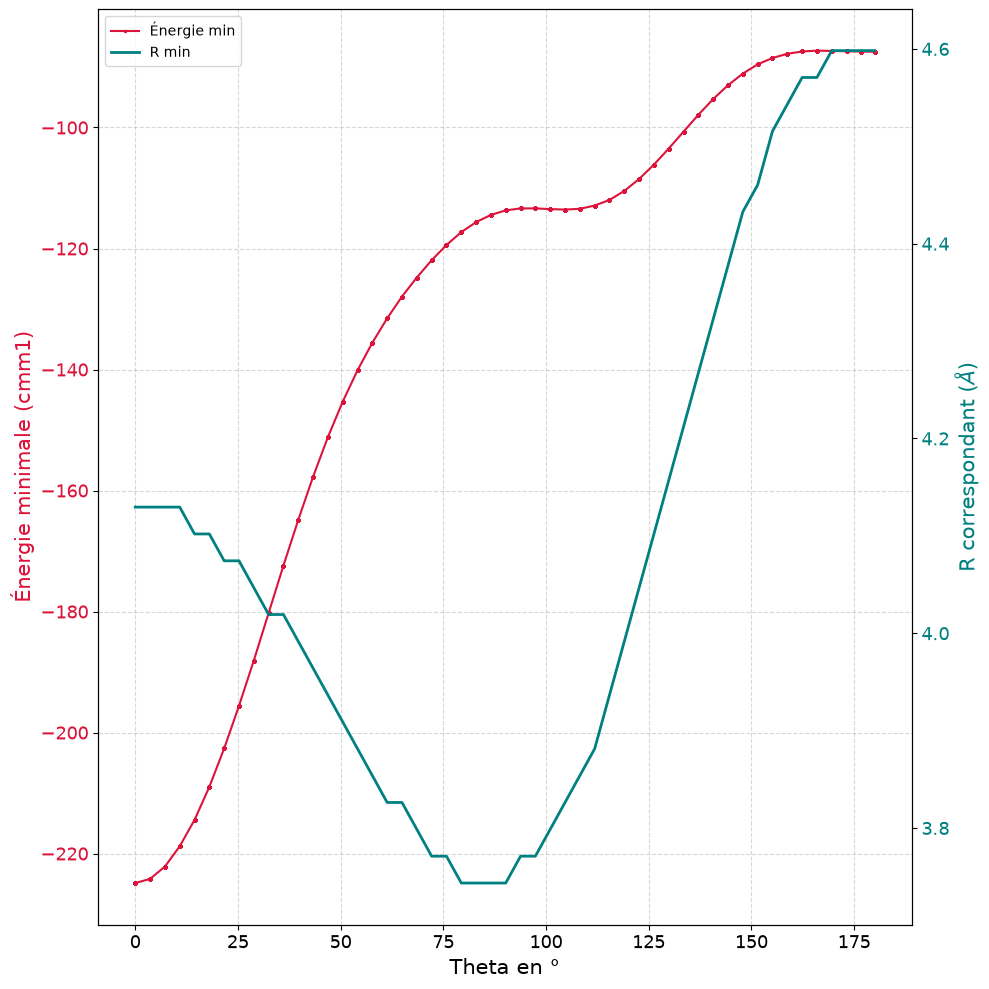
\includegraphics[width=\linewidth]{../Figures/HNC/MEP2.png}
    \end{subfigure}
    \begin{subfigure}{0.49\textwidth}
        \centering
        \caption{Paramètres \ref{params_ls_bounded}}
        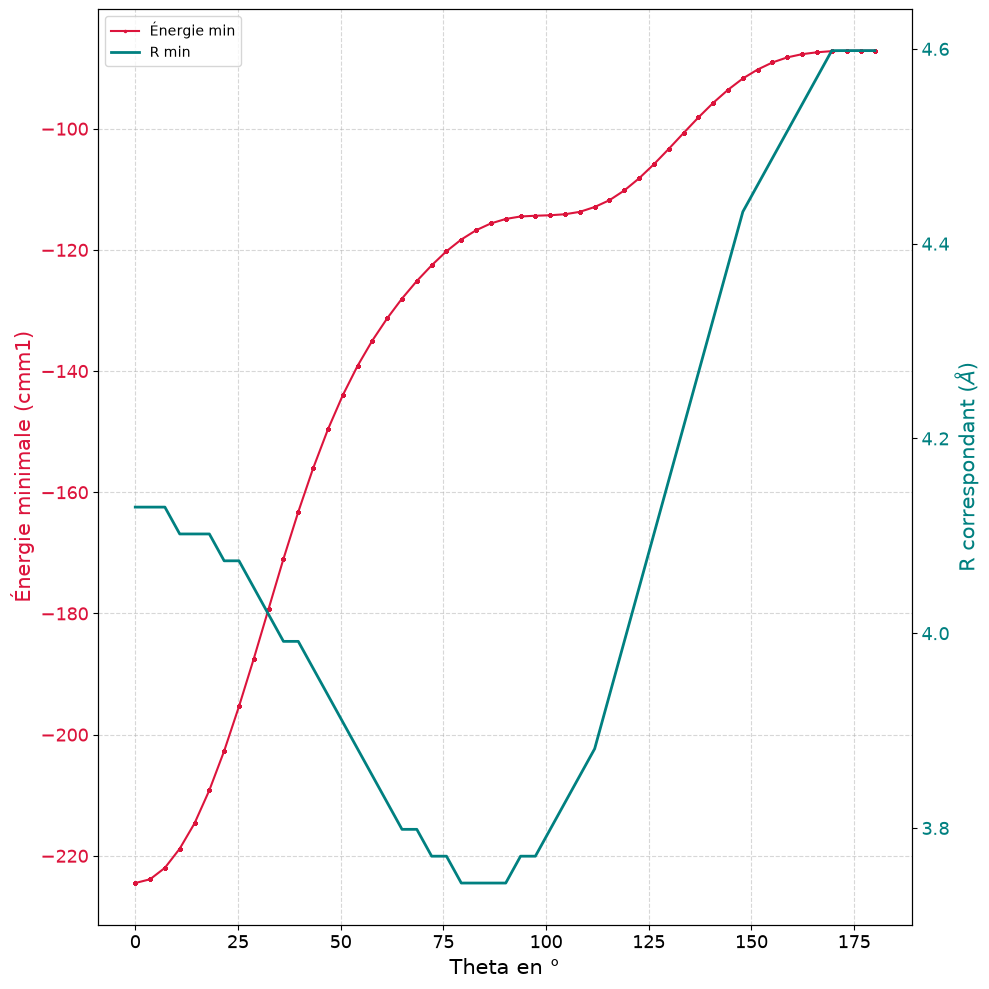
\includegraphics[width=\linewidth]{../Figures/HNC/MEP3.png}
    \end{subfigure}
\end{figure}

\newpage{}
\section{Courbes d'énergies potentielles pour $\theta$ fixé}

\begin{figure}[h]
    \centering
    \caption{Courbes d'énergies potentielles en cm$^{-1}$ avec Ar--HNC linéaire quand $\theta=0$°}
    \begin{subfigure}{0.45\textwidth}
        \centering
        \caption{$\theta=0$°}
        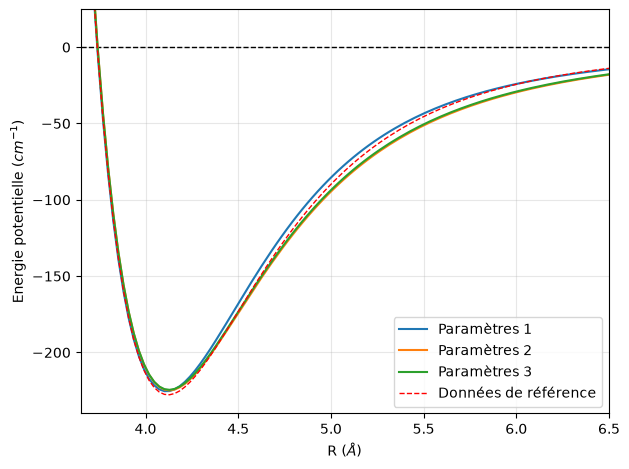
\includegraphics[width=\linewidth]{../Figures/HNC/courbeT0.png}
    \end{subfigure}
    \begin{subfigure}{0.45\textwidth}
        \centering
        \caption{$\theta=65$°}
        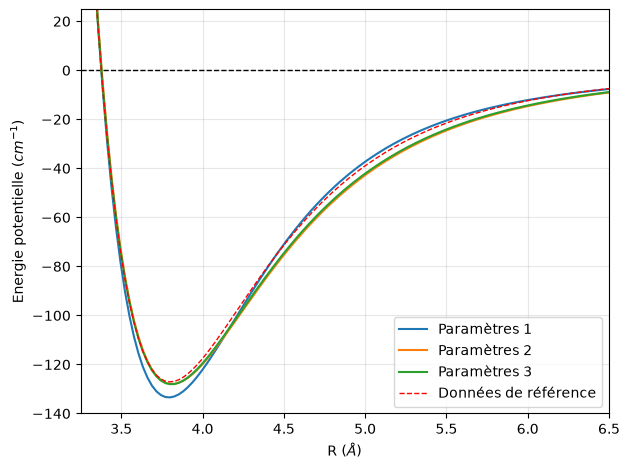
\includegraphics[width=\linewidth]{../Figures/HNC/courbeT65.png}
    \end{subfigure}
    \begin{subfigure}{0.45\textwidth}
        \centering
        \caption{$\theta=90$°}
        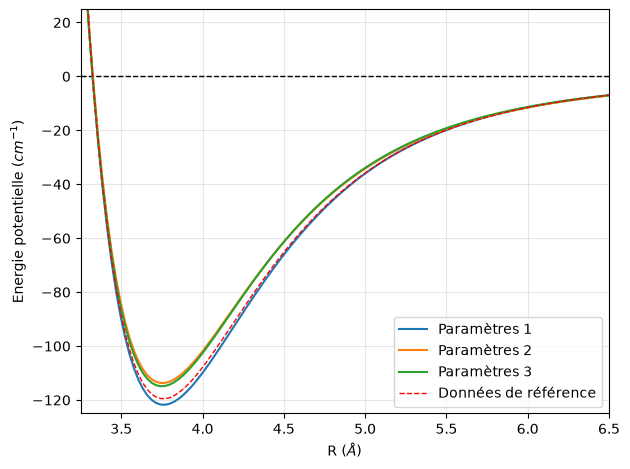
\includegraphics[width=\linewidth]{../Figures/HNC/courbeT90.png}
    \end{subfigure}
    \begin{subfigure}{0.45\textwidth}
        \centering
        \caption{$\theta=126$°}
        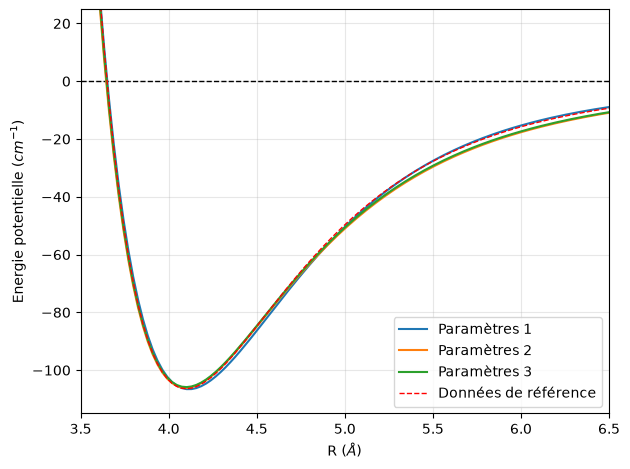
\includegraphics[width=\linewidth]{../Figures/HNC/courbeT126.png}
    \end{subfigure}
    \begin{subfigure}{0.45\textwidth}
        \centering
        \caption{$\theta=180$°}
        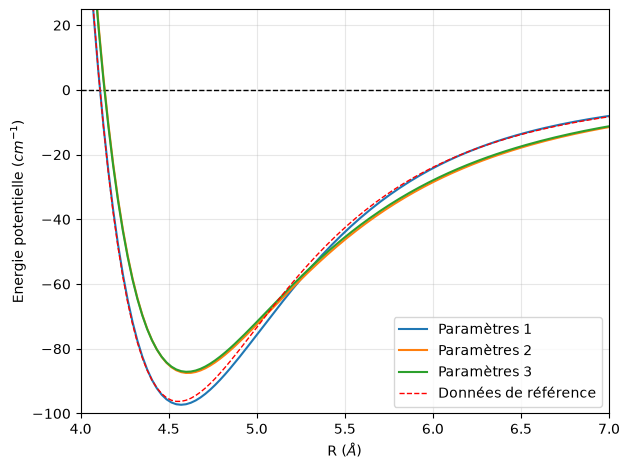
\includegraphics[width=\linewidth]{../Figures/HNC/courbeT180.png}
    \end{subfigure}
\end{figure}

\newpage{}
\section{Courbes d'énergies potentielles pour $R$ fixé}

\begin{figure}[h]
    \centering
    \caption{Courbes d'énergies potentielles en cm$^{-1}$ avec Ar--HNC linéaire quand $\theta=0$°}
    \begin{subfigure}{0.45\textwidth}
        \centering
        \caption{$R=2.92$ \AA}
        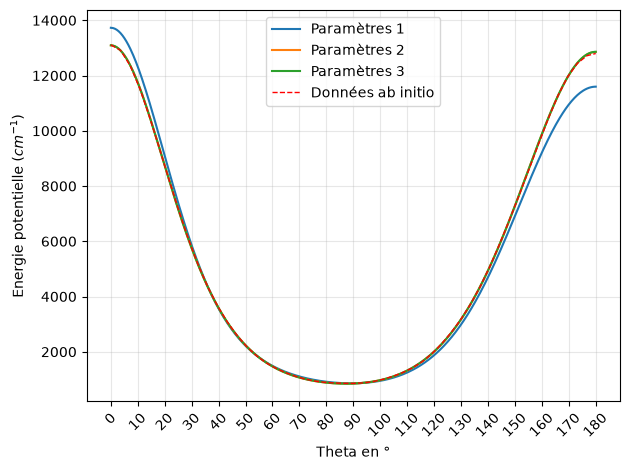
\includegraphics[width=\linewidth]{../Figures/HNC/courbeR292.png}
    \end{subfigure}
    \begin{subfigure}{0.45\textwidth}
        \centering
        \caption{$R=3.77$ \AA}
        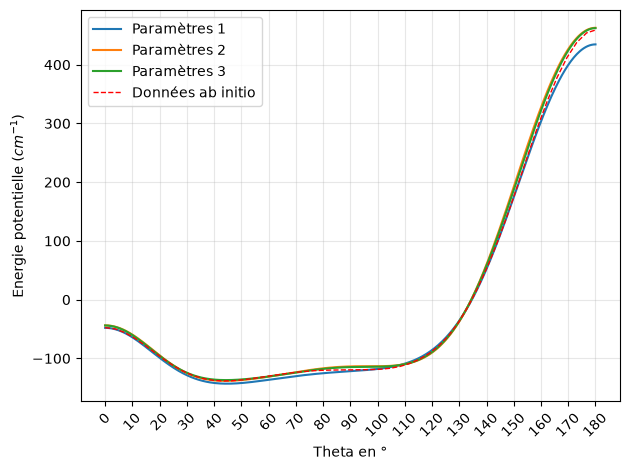
\includegraphics[width=\linewidth]{../Figures/HNC/courbeR377.png}
    \end{subfigure}
    \begin{subfigure}{0.45\textwidth}
        \centering
        \caption{$R=4.60$ \AA}
        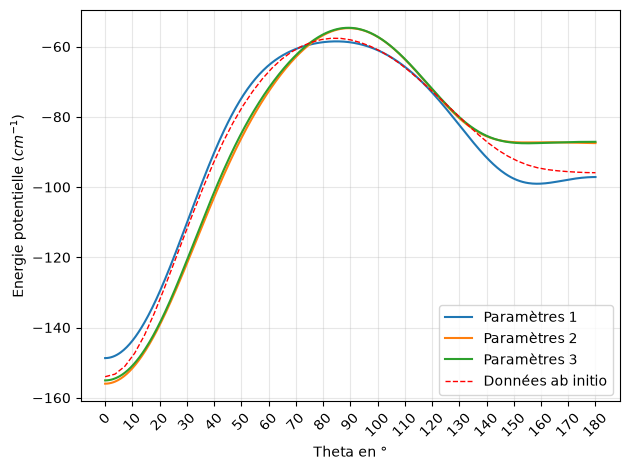
\includegraphics[width=\linewidth]{../Figures/HNC/courbeR460.png}
    \end{subfigure}
    \begin{subfigure}{0.45\textwidth}
        \centering
        \caption{$R=6.25$ \AA}
        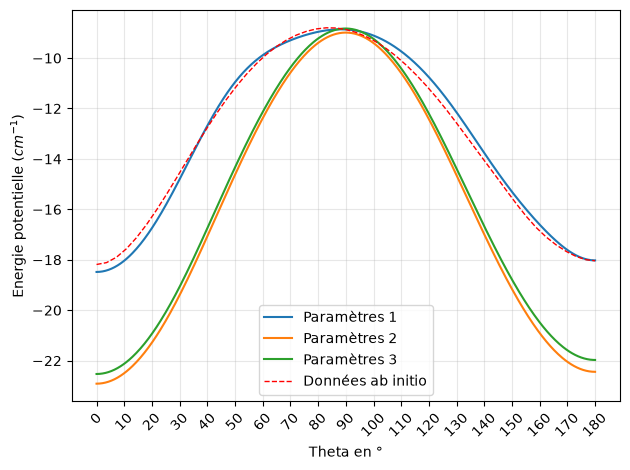
\includegraphics[width=\linewidth]{../Figures/HNC/courbeR625.png}
    \end{subfigure}
\end{figure}

\section{Conclusion}

Le jeu \ref{params_cf_trf_sigma} présente des métriques globales moyennes notament en raisons des erreurs importantes
dans les zones répulsives et pour les $\theta$ extrèmes.\\
Les jeux \ref{params_ls_sigma_final} et \ref{params_ls_bounded} sont meilleurs
sur l'ensemble des données avec des métriques globales bien plus bonnes. En 
revanche, ils perdent en précision dans la zone du puits et quand $R$ est grand.
Parmi les deux, je choisirai \ref{params_ls_bounded} . En raison de ses valeurs de 
\textbf{c} ainsi que pour sa régularité (voir Score de Régularité Table \ref{erreurs_global})\\

Le jeu de paramètres \ref{params_cf_trf_sigma} apporte plus de précisions
sur les minimums et les énergies attractives en général.\\

Le jeu de paramètres \ref{params_ls_bounded} est meilleur si on s'interesse
à la totalité des $R$ et $\theta$.

%--------------------------------------------------
\clearpage{}
\newpage{}
\appendix

\section{Figures complémentaires}

\begin{table}[ht]
\centering
\caption{Erreurs pour tous les paramètres calculés}
\label{erreurs_all}
\resizebox{\textwidth}{!}{%

\begin{tabular}{lrrrrrrrr}
\toprule
 & R² & RMSE (cm-1) & MAE (cm-1) & Relative Max (\%) & Relative Moyenne (\%) & Absolue Max (cm-1) & Absolue Moyenne (cm-1) & Score Régularité \\
\midrule
params\_opt\_cf\_lm & 0.999911 & 107.770322 & 22.851256 & 4.883434 & 0.189255 & 4967.183194 & 22.851256 & 2298 \\
params\_opt\_cf\_lm\_sigma & 0.973728 & 1849.431445 & 124.371681 & 42.103508 & 0.182533 & 104515.794564 & 124.371681 & 65 \\
params\_opt\_cf\_trf & 0.999903 & 112.381594 & 17.219203 & 5.199505 & 0.104209 & 5170.691283 & 17.219203 & 193 \\
params\_opt\_cf\_trf\_sigma & 0.975292 & 1793.545540 & 136.890764 & 38.508793 & 0.243320 & 98073.349786 & 136.890764 & 83 \\
params\_opt\_cf\_trf\_sigma\_A & 0.999818 & 154.119365 & 13.436969 & 6.226824 & 0.037949 & 6260.156793 & 13.436969 & 87 \\
params\_opt\_cf\_trf\_sigma\_B & 0.195193 & 10236.178747 & 1178.452880 & 4617.446791 & 15.348944 & 346411.066480 & 1178.452880 & 4527 \\
params\_opt\_cf\_trf\_sigma\_C & 0.989025 & 1195.343977 & 96.298408 & 20.437628 & 0.138792 & 57428.027060 & 96.298408 & 585 \\
params\_opt\_cf\_trf\_sigma\_good & 0.999864 & 133.234280 & 13.020100 & 5.411646 & 0.050063 & 5983.002643 & 13.020100 & 84 \\
params\_opt\_cf\_trf\_sigma\_hybrid & 0.999583 & 233.018557 & 16.376920 & 5.522550 & 0.052149 & 15591.792122 & 16.376920 & 88 \\
params\_opt\_ls & 0.999903 & 112.381594 & 17.219203 & 5.199505 & 0.104209 & 5170.691283 & 17.219203 & 193 \\
params\_opt\_ls\_jac & 0.999911 & 107.770318 & 22.849997 & 4.883627 & 0.189239 & 4967.035999 & 22.849997 & 2289 \\
params\_opt\_ls\_jac\_soft & 0.999899 & 114.916100 & 14.475609 & 5.481269 & 0.097738 & 5759.469574 & 14.475609 & 268 \\
params\_opt\_ls\_jac\_huber & 0.999897 & 115.549439 & 14.624066 & 5.497618 & 0.100200 & 5800.840485 & 14.624066 & 276 \\
params\_opt\_ls\_norm & 0.999874 & 127.890615 & 13.016173 & 5.941372 & 0.044654 & 5955.049264 & 13.016173 & 95 \\
params\_opt\_ls\_jac\_norm & 0.999014 & 358.208353 & 34.088310 & 6.532113 & 0.092588 & 19996.030735 & 34.088310 & 82 \\
params\_opt\_ls\_jac\_soft\_norm & 0.999952 & 78.993863 & 9.518621 & 2.984077 & 0.039665 & 3393.960213 & 9.518621 & 68 \\
params\_opt\_ls\_jac\_huber\_norm & 0.999953 & 78.620404 & 9.542489 & 2.987975 & 0.039935 & 3369.021869 & 9.542489 & 68 \\
params\_opt\_ls\_norm2 & 0.923751 & 3150.724970 & 502.888460 & 43.221783 & 1.531591 & 47892.630790 & 502.888460 & 424 \\
params\_opt\_ls\_jac\_norm2 & 0.777376 & 5383.663940 & 517.655621 & 167.117690 & 1.095600 & 220692.826797 & 517.655621 & 108 \\
params\_opt\_ls\_jac\_soft\_norm2 & 0.810597 & 4965.756237 & 445.386634 & 156.891232 & 1.109225 & 215435.781260 & 445.386634 & 89 \\
params\_opt\_ls\_jac\_huber\_norm2 & 0.824803 & 4775.898477 & 472.401123 & 136.912247 & 1.231363 & 203855.873980 & 472.401123 & 232 \\
params\_ls\_hybrid & 0.999298 & 302.245361 & 22.663976 & 6.508784 & 0.111057 & 21556.728980 & 22.663976 & 622 \\
params\_ls\_smooth & 0.999776 & 170.650213 & 18.613246 & 6.378620 & 0.095817 & 8765.122988 & 18.613246 & 283 \\
params\_ls\_sigma\_final & 0.999838 & 145.416083 & 12.418732 & 6.040209 & 0.037614 & 6843.420117 & 12.418732 & 81 \\
params\_ls\_bounded & 0.999820 & 153.207453 & 12.285500 & 6.815061 & 0.034710 & 7665.298152 & 12.285500 & 74 \\
\bottomrule
\end{tabular}%
}
\end{table}


%--------------------------------------------------
\bibliographystyle{plain}
\bibliography{references}

\end{document}
